% \documentclass[aspectratio=169,10pt,dvipsnames]{beamer} 
\usepackage{graphicx}
\usepackage{tabularx}
\usepackage{array}
\usepackage[most]{tcolorbox}
\usepackage{mathtools}
\usepackage{stackengine}
\usepackage{algorithmic}
\usepackage{epstopdf}
\usepackage{lipsum}
\usepackage{pifont}
\usepackage{algorithm}
\usepackage{tikz}
\usepackage{animate}
\usetikzlibrary{decorations.pathreplacing}
\usepackage[export]{adjustbox}
\renewcommand{\thealgorithm}{}
\usetikzlibrary{matrix}
\usepackage{natbib} 
\usepackage{bibentry}
\newcommand{\amin}{\mathop{\text{argmin}}}
\newcommand{\forestgreen}{\color{forestgreen}}
\newcommand{\red}{\color{red}}
\newcommand{\blue}{\color{blue}}
\newcommand{\bx}{\boldsymbol{x}}
\newcommand{\blambda}{\boldsymbol{\lambda}}
\newcommand{\by}{\boldsymbol{y}}
\newcommand{\bz}{\boldsymbol{z}}
\newcommand{\bX}{\boldsymbol{X}}
\newcommand{\bY}{\boldsymbol{Y}}
\newcommand{\bZ}{\boldsymbol{Z}}
\newcommand{\bv}{\boldsymbol{v}}
\newcommand{\bu}{\boldsymbol{u}}
\newcommand{\bxi}{\boldsymbol{\xi}}
\newcommand{\bpsi}{\boldsymbol{\psi}}
\newcommand{\bzeta}{\boldsymbol{\zeta}}
\newcommand{\boldsymbolu}{\boldsymbol{\mu}}
\newcommand{\bQ}{\boldsymbol{Q}}
\newcommand{\bS}{\boldsymbol{S}}
\newcommand{\bT}{\boldsymbol{T}}
\newcommand{\bF}{\boldsymbol{F}}
\newcommand{\bG}{\boldsymbol{G}}
\newcommand{\bd}{\boldsymbol{d}}
\newcommand{\bp}{\boldsymbol{p}}
\newcommand{\bff}{\boldsymbol{f}}
\newcommand{\bc}{\boldsymbol{c}}
\newcommand{\bg}{\boldsymbol{g}}
\newcommand{\bA}{\boldsymbol{A}}
\newcommand{\bB}{\boldsymbol{B}}
\newcommand{\bSigma}{\boldsymbol{\Sigma}}
\newcommand{\bC}{\boldsymbol{C}}
\newcommand{\bE}{\boldsymbol{E}}
\newcommand{\bh}{{\boldsymbol{h}}}
\newcommand{\bH}{{\boldsymbol{H}}}
\newcommand{\bJ}{{\boldsymbol{J}}}
\newcommand{\bR}{{\boldsymbol{R}}}
\newcommand{\bn}{\boldsymbol{n}}
\newcommand{\br}{\boldsymbol{r}}
\newcommand{\bl}{\boldsymbol{l}}
\newcommand{\bI}{\boldsymbol{I}}
\newcommand{\bzero}{\boldsymbol{0}}
\newcommand{\st}{\mathop{\text{s.t.}}}
\newcommand{\diag}{\mathop{\text{\normalfont diag}}}
\newcommand{\aminmax}{\mathop{\text{\normalfont argminmax}}}
\newcommand{\interior}{\mathop{\text{\normalfont interior}}}
\newcommand{\ReH}{\mathop{\text{\normalfont Re}}}

\setbeamertemplate{navigation symbols}{}

\newcommand\blfootnotefirst[1]{%
  \begingroup
  \renewcommand\thefootnote{}\footnote{\color{darkgray}\tiny\vspace{-.13in}\hspace{-.32in}#1}%
  \addtocounter{footnote}{-1}%
  \endgroup
}

\newcommand\blfootnote[1]{%
  \begingroup
  \renewcommand\thefootnote{}\footnote{\color{darkgray}\tiny\vspace{-.02in}\hspace{-.32in}#1}%
  \addtocounter{footnote}{-1}%
  \endgroup
}

\newcommand\with[1]{%
  \begingroup
  \renewcommand\thefootnote{}\footnote{\hspace{-.32in}\normalfont Joint Work with #1}%
  \addtocounter{footnote}{-1}%
  \endgroup
}
\renewcommand\footnoterule{}

%% Colors
\definecolor{forestgreen}{rgb}{0.13, 0.55, 0.13}
\definecolor{green2}{rgb}{0, 0.8, 0}
\definecolor{UWGray}{RGB}{90,90,90}
\definecolor{UWRed}{RGB}{38,72,161}
\setbeamerfont{author}{series=\bfseries}
\setbeamerfont{title}{series=\bfseries}
\setbeamerfont{frametitle}{series=\bfseries}
\setbeamerfont{block title}{size={}}
\setbeamercolor{block title}{fg=UWRed}
\newcommand{\green}{\color{green2}}
\newcommand{\UWgray}{\color{UWGray}}
\newcommand{\UWred}{\color{UWRed}}
\usepackage{cmbright}
% \usefonttheme{professionalfonts} % using non standard fonts for beamer
% \usepackage[utf8]{inputenc} 
% \usepackage[T1]{fontenc}
% \usepackage[frenchb]{babel}
% \usepackage{setspace}
\usepackage{color}
\usepackage{listings}
\lstdefinelanguage{Julia}%
{morekeywords={abstract,break,case,catch,const,continue,do,else,elseif,%
end,export,false,for,function,immutable,import,importall,if,in,%
macro,module,otherwise,quote,return,switch,true,try,type,typealias,%
using,while,@threads,@optinode,@variable,@constraint,@NLnodeconstraint,@linkconstraint,@objective,@optiedge},%
sensitive=true,%
alsoother={$},%$
morecomment=[l]\#,%
morecomment=[n]{\#=}{=\#},%
morestring=[s]{"}{"},%
morestring=[m]{'}{'},%
}[keywords,comments,strings]%
\definecolor{codegreen}{rgb}{0,0.6,0}
\definecolor{codegray}{rgb}{0.5,0.5,0.5}
\definecolor{codepurple}{rgb}{0.58,0,0.82}
\definecolor{backcolour}{rgb}{0.95,0.95,0.92}
\lstdefinestyle{mystyle}{
backgroundcolor=\color{backcolour},   
commentstyle=\color{codegreen},
keywordstyle=\color{magenta},
numberstyle=\tiny\color{codegray},
stringstyle=\color{codepurple},
basicstyle=\ttfamily\footnotesize,
breakatwhitespace=false,         
breaklines=true,                 
captionpos=b,                    
keepspaces=true,                 
numbers=left,                    
numbersep=5pt,                  
showspaces=false,                
showstringspaces=false,
showtabs=false,                  
tabsize=2
}
\lstset{%
language         = Julia,
basicstyle       = \ttfamily,
keywordstyle     = \bfseries\color{blue},
stringstyle      = \color{magenta},
commentstyle     = \color{ForestGreen},
showstringspaces = false,
style            = mystyle
}

\usepackage{pgfplots}
\usepackage{tikz}
\usetikzlibrary{calc}
\usetikzlibrary{colorbrewer}
\pgfplotsset{colormap/blackwhite}

\tikzset{%
  add/.style args={#1 and #2}{to path={%
 ($(\tikztostart)!-#1!(\tikztotarget)$)--($(\tikztotarget)!-#2!(\tikztostart)$)%
  \tikztonodes}}
} 

\beamersetrightmargin{0.025\paperwidth}
\beamersetleftmargin{0.025\paperwidth}

\usepackage{animate}


\definecolor{emph}{rgb}{0.2,0.2,0.7}
\setbeamertemplate{footline}[frame number]
\setbeamertemplate{subsection in toc}{\hspace*{2em}{\footnotesize \inserttocsectionnumber.\inserttocsubsectionnumber.~\inserttocsubsection\par}}
\setbeamertemplate{section in toc}{\inserttocsectionnumber.~\inserttocsection\par}
\usepackage{hyperref}

\usepackage{times}
\usepackage{DejaVuSansMono}

\usepackage{enumitem}
\setitemize{label=\usebeamerfont*{itemize item}%
  \usebeamercolor[fg]{itemize item}
  \usebeamertemplate{itemize item}}

\newcommand{\backupbegin}{
   \newcounter{finalframe}
   \setcounter{finalframe}{\value{framenumber}}
}
\newcommand{\backupend}{
   \setcounter{framenumber}{\value{finalframe}}
}
\usetikzlibrary{positioning, fadings, backgrounds}

\usepackage{multirow}
\newcommand{\reference}[1]{%
  \tikz[remember picture,overlay,align=center]{s
    \node[anchor=south west,color=darkgray,font=\tiny,align=left,inner sep=1] at (current page.south west) {#1};
  }%
}
\title{Accelerating Optimal Power Flow with GPUs: SIMD Abstraction of Nonlinear Programs and Condensed-Space Interior-Point Methods 
}

\author{
  \IEEEauthorblockN{Sungho Shin and Mihai Anitescu}
  \IEEEauthorblockA{
    Mathematics and Computer Science Division\\
    Argonne National Laboratory\\
    Lemont, IL, USA\\
    sshin@anl.gov, anitescu@mcs.anl.gov}
  \and
  \IEEEauthorblockN{François Pacaud}
  \IEEEauthorblockA{Centre Automatique et Systèmes\\
    Mines Paris - PSL \\
    Paris, France\\
    francois.pacaud@minesparis.psl.eu}
}

\date{\small
  $^{1}$Mathematics and Computer Science Division, Argonne National Laboratory\\
  $^{2}$Centre Automatique et Syst\`{e}mes, Mines Paris - PSL
}
\begin{document}
\maketitle
\begin{abstract}
  This paper introduces a novel computational framework for efficiently
  solving AC optimal power flow (OPF) problems using GPUs. Although GPUs
  have demonstrated remarkable performance in various computing domains,
  their application in AC OPF has been limited due to challenges such as
  serial computations for automatic differentiation (AD) and sparse matrix
  factorization. To address these obstacles, we propose two strategies.
  First, we utilize a single-instruction, multiple-data (SIMD)
  abstraction of nonlinear programs (NLP). This approach allows us to
  specify model equations while preserving their parallelizable
  structure. By implementing AD on GPUs
  efficiently, we can fully leverage the computational power of these
  devices.  Second, we employ a Condensed-Space Interior-Point Method
  (IPM) with inequality relaxation. This technique involves relaxing
  equality constraints to inequalities and condensing the
  Karush-Kuhn-Tucker system to the primal space. As a result, we enable
  efficient sparse matrix factorization on GPUs without requiring a
  numerical pivoting procedure.  By combining these strategies, we
  achieve efficient AC OPF problem solutions on GPUs, keeping the
  problem data residing in the device memory and performing the majority
  of computations on the GPUs. Comprehensive numerical benchmark results
  showcase the substantial computational advantage of our approaches for
  solving AC OPF problems up to moderate precision on NVIDIA
  GPUs. Remarkably, our method achieves an order of magnitude speedup
  compared to state-of-the-art tools on CPUs, such as JuMP.jl, AMPL, and
  Ipopt. The paper concludes by discussing the future extensibility of
  our method.
\end{abstract}


\section{Introduction}

While graphics processing units (GPUs) have demonstrated remarkable
capabilities in various computing domains, their adoption in
large-scale constrained nonlinear optimization regimes, such as
alternating current (AC) optimal power flow (OPF) problems, has faced
some limitations. One of the primary challenges arises from the
automatic differentiation (AD) of sparse model equations and the parallel
factorization of indefinite sparse matrices commonly encountered
within constrained optimization algorithms
\cite{anitescu2021targeting}. While GPU computation can trivially
accelerate several parts of the optimization process, especially
various internal computations within the optimization solver, the
sluggish data transfer between host and device memory hampers the
ad-hoc implementation of GPU accelerations (Fig. \ref{fig:simd}). To
fully leverage the potential that modern GPU hardware has to offer, it
becomes imperative to have a comprehensive computational framework for
optimization on GPUs so that AD, linear algebra
operations, and optimization can be performed entirely on the GPU.
Specifically, for best performance, both the problem data and the
solver's intermediate computational data must be exclusively resident
within the device memory, with the majority of operations executed on
the GPU.

\begin{figure}[t]
  \centering
  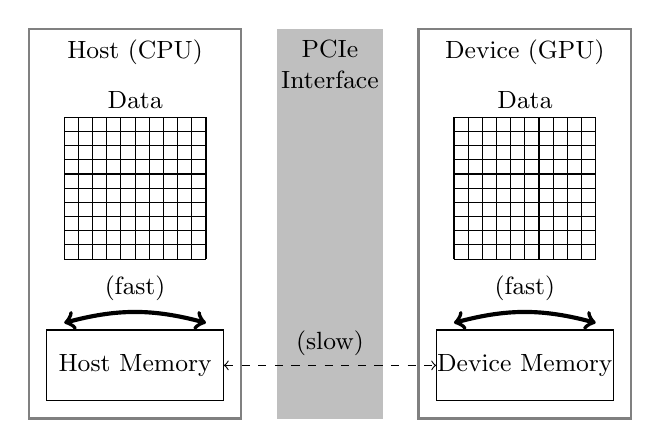
\begin{tikzpicture}[remember picture, scale=.9, font=\small]

    \fill[lightgray] (3.25,-.75) rectangle (4.75,4.75) node[black,midway,align=center,yshift=57.5] {PCIe\\Interface};
    \draw[gray,thick] (-.25,-.75) rectangle (2.75,4.75) node[black,midway,align=center,yshift=62] {Host (CPU)};
    \draw[gray,thick] (5.25,-.75) rectangle (8.25,4.75) node[black,midway,align=center,yshift=62] {Device (GPU)};

    \node[align=center] at (1.25, 3.75) {Data};
    \node[align=center] at (6.75, 3.75) {Data};

    % Host Memory
    \draw (0,-.5) rectangle (2.5,.5) node[midway] {Host Memory};

    % Device Memory
    \draw (5.5,-.5) rectangle (8,.5) node[midway] {Device Memory};


    % Arrow with Dashed Line
    \draw[<->, dashed] (2.5, 0) -- (5.5, 0) node[midway, above, align=center] {(slow)};
    \draw[<->, line width=1.5] (.25, .6) to [in=165, out =15] node[midway, above, align=center] {(fast)}(2.25, .6) ;
    \draw[<->, line width=1.5] (5.75, .6) to [in=165, out =15] node[midway, above, align=center] {(fast)}(7.75, .6) ;

    \def\rows{10}
    \def\cols{10}
    \def\elementwidth{2}
    \foreach \xshift/\yshift in {.25/1.5, 5.75/1.5} {

      % Draw Grid
      \foreach \i in {0,...,\rows} {
        \draw (\xshift, \yshift+\i*\elementwidth/\rows) -- (\xshift+\elementwidth, \yshift+\i*\elementwidth/\rows);
      }
      \foreach \i in {0,...,\cols} {
        \draw (\xshift+\i*\elementwidth/\cols, \yshift) -- (\xshift+\i*\elementwidth/\cols, \yshift+\elementwidth);
      }
    }
  \end{tikzpicture}
  \caption{A schematic description of host (CPU) and device (GPU) memory.}\label{fig:memory}
\end{figure}

This paper presents our approach to implement a comprehensive
computational framework for solving large-scale 
OPF problems on NVIDIA GPUs, along with the associated software
implementations: SIMDiff.jl, an AD tool, and
MadNLP.jl, a nonlinear optimizaiton solver. Our approach incorporates
two novel strategies: (i) a single-instruction, multiple-data (SIMD)
abstraction of nonlinear programs (NLPs), enabling streamlined
parallel AD on GPUs, and (ii) a condensed-space
interior-point method (IPM) with an inequality relaxation strategy,
which facilitates the use of highly efficient {\it refactorization}
routines for sparse matrix factorization with fixed pivot sequences.

While derivative evaluation can be generally cheaper than linear
algebra operations, our numerical results show that AD often
constitutes more than half of the total solver time when using
off-the-shelf AD implementations like JuMP.jl or AMPL. Instead of the
general-purpose tools, our method leverages a specialized AD
implementation based on the SIMD abstraction of NLPs. This abstraction
alllows to preserve the parallelizable structure within the model
equations, facilitating efficient derivative evaluations on the
GPU. The AC power flow model is particularly well-suited for this
abstraction as it involves repetitive expressions for each component
type (e.g., buses, lines, generators), and the number of computational
patterns does not increase with the network's size. Numerical results
reported in this paper demonstrate that our proposed strategies can
achieve over 20 times speedup. In comparison to general AD implementations
on CPUs (such as AMPL and JuMP.jl), our GPU-based method is
approximately 50 times faster in the largest instances.

Linear algebra operations, especially sparse indefinite matrix
factorization, are typically the bottleneck in nonlinear optimization
solvers. Parallelizing this operation is challenging due to the need
for numerical pivoting, which ensures the numerical
stability. However, when the matrix can be factorized without
numerical pivoting, a significant part of the operation can be
parallelized, and the numerical factorization can be efficiently
performed on GPUs. We develop a condensed-space IPM strategy that
allows the use of sparse matrix factorization routines without
numerical pivoting. This strategy relaxes equality constraints by
permitting small violations, which enables expressing the
Karush-Kuhn-Tucker (KKT) system entirely in the primal space
through the condensation procedure. Although this strategy is not new
\cite{nocedal2006numerical}, it has traditionally been considered less
efficient than the standard full-space method due to increased nonzero
entries in the KKT system. However, when implemented on GPUs, it
offers the key advantage of ensuring positive definiteness in the
condensed KKT system through the application of standard
regularization techniques. This, in turn, allows for the utilization
of linear solvers with a fixed numerical pivot sequence (known as
refactorization). An efficient implementation of sparse
refactorization is available as part of the CUDA library, enabling the
implementation of efficient KKT system solutions on GPUs. Although
this method is susceptible to numerical stability issues due to
increased condition number in the KKT system, our results demonstrate
that the solver is robust enough to solve problems with a relative
accuracy of $\epsilon_{\text{mach}}^{1/4}\approx 10^{-4}$.

We present numerical benchmark results to showcase the efficiency of
our proposed approach, utilizing two of our packages: MadNLP.jl and
SIMDiff.jl. The solution of the KKT system is performed using the
external cuSOLVER library. To assess the performance of our method, we
compare it against standard CPU approaches using the widely used data
available in pglib-opf \cite{wachter2006implementation}.  Our
benchmark results demonstrate that our proposed computational
framework has significant potential for accelerating the solution of
AC OPF problems, particularly for large-scale instances, especially
when a moderate tolerance (e.g., $10^{-4}$) is
considered. Specifically, when running on NVIDIA GPUs, our method
achieves a notable 4x speedup compared to our solver running on CPU,
in the case of the largest instance. Moreover for the same instance,
our approach surpasses the performance of existing tools (such as
Ipopt interfaced with JuMP.jl) by an order of magnitude.  This finding
underscores the importance of harnessing the computational power of
GPUs as a key enabler for tackling the challenges posed by large-scale
OPF problems. 


\paragraph*{Organization}
The paper is organized as follows. In the remainder of the current
section, we introduce the mathematical notation. In Section
\ref{sec:prelim}, we provide general preliminary knowledge on
numerical optimization and GPU computing. In Section \ref{sec:simd},
we present the SIMD abstraction strategy for large-scale nonlinear
programs and their advantages in terms of implementing parallel
AD. Section \ref{sec:ipm} presents the
optimization algorithm under study, the condensed-space interior point
method with inequality relaxation strategy. Section \ref{sec:num}
presents the numerical results, comparing our approach with other
state-of-the-art solution methods on GPUs. Finally, conclusions and
future outlooks are given in Section \ref{sec:conc}.

\paragraph*{Notation}
We denote the set of real numbers and the set of integers by
$\mathbb{R}$ and $\mathbb{I}$. We let $[M]:=\{1,2,\cdots,M\}$. We let
$[v_i]_{i\in[M]}:=[v_1;v_2;\cdots,v_M]$.  A vector of ones with an
appropriate size is denoted by $\boldsymbol{1}$. We use the following
convention for any symbol $x$: $X:=\diag(x)$.

\section{Preliminaries}\label{sec:prelim}
This section covers three essential background topics: numerical
optimization, AD, and GPU computing.

\subsection{Numerical Optimization}\label{sec:numopt}
We consider NLPs of the form:
\begin{subequations}\label{eqn:cpt}
  \begin{align}
    \min_{x^\flat \leq x \leq x^\sharp}\;
    & f(x)\\
    \st\;
    & g(x) =0. \label{eqn:cpt-con}
  \end{align} 
\end{subequations}
Numerous solution algorithms have been developed in the NLP
literature.  These methods can be broadly classified into active-set
methods and interior-point methods \cite{nocedal2006numerical}.
Active-set methods aim to find the set of active consraints associated
with the optimal solution in a combinatorial manner, while
interior-point methods replace inequality constraints with smooth
barrier functions, enabling the use of Newton-type second-order
algorithms. Interior-point methods are known to be more scalable for
problems with a large number of constraints and suitable for
parallelization, thanks to the fixed sparsity pattern of the KKT
matrix. We adopt the interior-point approach and develop our
optimizationmethods on GPUs.

In terms of practical computations, three key components play
vital roles: derivative evalutions (often provided by the AD
capabilities of the algebraic modeling languages), linear algebra
operations, and internal computations within the solver. Notably, most
of the computational efforts are delegated to the external linear
solver and AD library. The optimization solver
orchestrates the operation of these tools to drive the solution
iterate towards the stationary point of the optimization problem, but
computations performed within the solver are generally much cheapr and
simpler compared to the operations in AD and linear solver packages.

Since the successful implementation of the open-source interior point
solver in Ipopt, many subsequent implementations of nonlinear
optimizaiton solvers
\cite{chiang2014structured,rodriguez2023scalable,shin2021graph} have
been based on Ipopt \cite{wachter2006implementation}. We also use
Ipopt as our main reference for the IPM implementation. Below, we
outline the overall computational procedure employed wihtin nonlinear
optimization frameworks:

1) Given the current primal-dual iterate $(x^{(\ell)},y^{(\ell)},
z^{\flat(\ell)},z^{\sharp(\ell)})$, the AD package computes:
$\nabla_x f(x^{(\ell)})$, $\nabla_x g(x^{(\ell)})$, $\nabla^2_{xx}
\mathcal{L}(x^{(\ell)},y^{(\ell)},z^{\flat(\ell)},z^{\sharp(\ell)})$, where
$\mathcal{L}(x^{\flat},y^{\flat},z^{\flat},z^{\sharp}):=f(x) - y^\top
g(x) - z^\flat (x-x^\flat) - z^\sharp (x^\sharp-x)$.

2) The following sparse indefinite system (known as the KKT system) is
solved using sparse indefinite factorization (typically, via sparse
LBL$^\top$ factorization) and triangular solve routines.
\begin{align}\label{eqn:kkt-indefinite}
  &\begin{bmatrix}
    W^{(\ell)}  + \Sigma^{(\ell)} + \delta^{(\ell)}_w I& A^{(\ell)\top}\\
    A^{(\ell)} & -\delta_c I\\
  \end{bmatrix}
  \begin{bmatrix}
    \Delta x\\
    \Delta y\\
  \end{bmatrix}=
  \begin{bmatrix}
    f - \mu X^{-1} \boldsymbol{1}\\
    \Delta y\\
  \end{bmatrix}
\end{align}
Here, $W^{(\ell)}:=\nabla^{2}_{xx}\mathcal{L}(x^{(\ell)},y^{(\ell)})$,
$A^{(\ell)}:= \nabla_xg(x^{(\ell)})$, and $\delta_w, \delta_c>0$ are
the regularization parameters determined based on the inertia
correction procedure.

3) The optimization solver employs the filter line search procedure to
determine the step size. While alternative approaches, such as
trust-region-type methods and merit function-based criteria, can be
used for determining the step size, the filter line search method is
most commonly used due to its implementation in Ipopt.

\subsection{AD}
Efficiently evaluating the derivatives of $f(\cdot)$, $g(\cdot)$, and
$\mathcal{L}(\cdot,\cdot)$ is crucial for the efficient solution of
optimization problems.

Numerical differentiation of computer programs can be achieved through
three different methods: (i) finite difference method, (ii) symbolic
differentiation, and (iii) AD. The finite difference method suffers
from numerical rounding errors, and its computational complexity grows
unfavorably with respect to the number of function arguments, making
it less preferable unless no other alternatives are
available. Symbolic differentiation uses computer algebra systems to
obtain symbolic expressions of first or higher-order
derivatives. While this method can differentiate functions up to high
numerical precision, it suffers from "expression swelling" effect and
struggles to compute the derivatives of long nested expressions in a
computationally efficient way.

In contrast, AD differentiates computer
programs by leveraging the computation graph. By inspecting the
computation graph and applying chain rules, AD
can efficiently and accurately evaluate derivatives. This approach has
become the dominant paradigm for derivative computation within the
scientific computing domain, including nonlinear optimization and
machine learning. For large-scale optimization, such as AC OPFs, AD
tools are often implemented as part of domain-specific modeling
languages, such as JuMP, CasADi, and AMPL (optimization) and Torch and
Flux (machine learning).

There are two alternative ways of propagating derivatives through the
recursive application of chain rules: (i) forward-mode and (ii)
reverse-mode, which operate in opposite directions (from leaves to
root and from root to leaves, respectively). Reverse-mode automatic
differentiation, also known as an adjoint method, has proven to be
particularly effective for dealing with the function expressions in
large-scale optimization problems.

The Julia Language, our language of choice, provides convenient ways
of implementing highly efficient automatic
differentiation. \textit{Any Julia function}, including commonly used
operations such as addition, multiplication, trigonometric functions,
exponential functions, and others, can be straightforwardly extended
through the use of multiple dispatch paradigm, allowing functions to
be dynamically dispatched based on the run-time type. Several
implementations of AD are available in Julia, including
ReverseDiff.jl, ForwardDiff.jl, Zygote.jl, and JuMP.jl. While these
tools are general and useful for various applications, they are not
optimized for evaluating derivatives of AC OPF problems, which contains
an obvious parallelizable structure that can be exploited.


\subsection{GPU Computing}\label{sec:gpu}
With the increasing prevalence of GPU in various scientific computing
tasks, there has been growing interest in leveraging these parallel
systems to efficiently solve large-scale OPF problems. Some recent
concurrent approaches include HyKKT, a hybrid (direct-iterative) KKT
system solver, \cite{regev2023hykkt} and HiOP, a HPC solver for
nonlinear optimization problems, \cite{hiop_techrep}. However,
adapting the IPM to GPUs presents challenges due to the fundamental
differences between GPU and CPU programming paradigms. While CPUs
execute a sequence of instructions on a single input (single
instruction, single data, or SISD, in Flynn's taxonomy), GPUs run the
same instruction simultaneously on hundreds of threads using the SIMD
paradigm (see Fig. \ref{fig:simd}). The SIMD parallelism works well
for algorithms that can be decomposed into simple instructions running
entirely in parallel, but not all algorithms seamlessly fit this
paradigm. For example, branching in the control flow can hinder
lockstep execution across multiple threads, and in turn, prevents
efficient implementations on GPUs. On the other hand, when the
algorithm's structure allows for efficient parallelization, the SIMD
parallelism in GPUs becomes highly effective, and oftentimes enables
orders of magnitudes speedup.

We highlight that the following, arguably quite common, computational
patterns are particularly effective when implemented on GPUs:
\begin{align}
  y&\leftarrow \left[g(x; q_j)\right]_{j\in [J]}\tag{Pattern 1}\label{eqn:pattern-1}\\
  y&\leftarrow y + \sum_{k\in [K]} h(x;s_k)\tag{Pattern 2}\label{eqn:pattern-2}\\
  o&\leftarrow \sum_{i\in [I]} f(x; p_i)\tag{Pattern 3}\label{eqn:pattern-3}.
\end{align}
Here, it is assumed that $f:\mathbb{R}^{n_x}\times
\mathbb{R}^{n_{p}}\rightarrow \mathbb{R}$, $g:\mathbb{R}^{n_x}\times
\mathbb{R}^{n_{s}}\rightarrow \mathbb{R}$, and
$h:\mathbb{R}^{n_x}\times \mathbb{R}^{n_{p}}\rightarrow
\mathbb{R}^{n_y}$ are simple instructions that require only a handful
of operations. \ref{eqn:pattern-1} is typically most effective on
GPUs, where each available thread can operate independently without
needing to simultaneously manipulate the same data reference in device
memory. \ref{eqn:pattern-2} and \ref{eqn:pattern-3} are more
challenging to implement, as they require simultaneous access to the
same device memory location, but they can be parallelized effectively
by using buffers.

Many of the operations required in AD of sparse
physical models, as well as the application of optimization
algorithms, are based on the computational patterns mentioned
above. For example, an OPF model can be implemented
with 14 different computational patterns, all of which fall within the
aforementioned categories. Additionally, the computation within
optimization solvers, such as forming the left-hand-side for the KKT
systems, computing the $\|\cdot\|_\infty$ norm of the constraint
violation, and assembling the condensed KKT system, can be carried out
by using these computational patterns. The only exception is the
factorization of the sparse KKT matrix, which requires more sophisticated
implementations.

Implementing kernel functions for the above computational patterns in
the Julia Language is straightforward, as it provides excellent
high-level interfaces for array and kernel programming for GPU
arrays. The code can even be device-agnostic, thanks to the portable
programming capability brought by KernelAbstractions.jl. All
of the AD and optimization capabilities in our
tools, MadNLP.jl and SIMDiff.jl, are implemented in Julia Language,
utilizing its kernel and array programming capabilities.

\begin{figure}[t]
  \centering 
  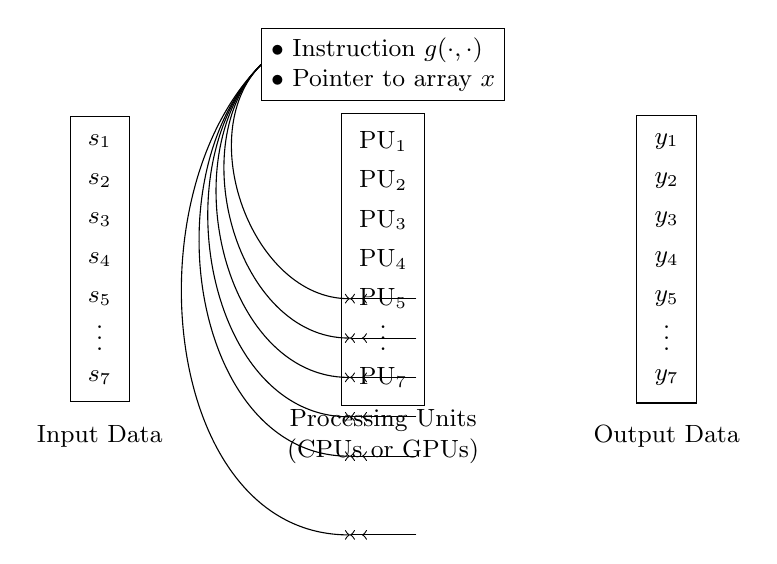
\begin{tikzpicture}[remember picture, scale=.9, font=\small]
    \node[draw,align=left] (I) at (0,2.75) {
      $\bullet$ Instruction $g(\cdot,\cdot)$\\
      $\bullet$ Pointer to array $x$
    };
    \node[draw] at (-4,0) {
      \tikz{
        \foreach\x in {1,2,3,4,5,7}{
          \node (A\x) at (0,-\x/2) {$s_{\x}$};
        }
        \node at (0,-2.9) {$\vdots$};
      }
    };
    \node[draw] at (0,0) {
      \tikz{
        \foreach\x in {1,2,3,4,5,7}{
          \node (B\x) at (0,-\x/2) {$\text{PU}_{\x}$};
        }
        \node at (0,-2.9) {$\vdots$};
      }
    };
    \node[draw] at (4,0) {
      \tikz{
        \foreach\x in {1,2,3,4,5,7}{
          \node (C\x) at (0,-\x/2) {$y_{\x}$};
        }
        \node at (0,-2.9) {$\vdots$};
      }
    };
    \foreach\x in {1,2,3,4,5,7}{
      \draw[->] (A\x.east) -- (B\x.west);
      \draw[->] (B\x.east) -- (C\x.west);
      \draw[->] (I.west) to [out=-135,in=180] (B\x.west);
    }
    \node at (-4,-2.5) {Input Data};
    \node[align=center] at (0,-2.5) {Processing Units\\(CPUs or GPUs)};
    \node at (4,-2.5) {Output Data};
  \end{tikzpicture}
  \label{fig:simd}
  \caption{A schematic description of SIMD parallelism in GPU computing}
\end{figure}

\section{SIMD Abstraction of NLPs}\label{sec:simd}

This section describes our implementation of SIMD abstraction and
sparse AD of the model equations. The abstraction and AD are
implemented as part of our algebriac modeling language SIMDiff.jl.

The SIMD abstraction under consideration is as follows:
\begin{subequations}\label{eqn:prob}
  \begin{align}
    \min_{x^L\leq x \leq x^U}& \sum_{\ell\in[L]}\sum_{i\in [I_k]} f^{(\ell)}(x; p^{(\ell)}_i)\\
    \st\; &\forall m\in[M]:\\
                             &\begin{aligned}[t]
                               g^{(m)}_\flat\leq &\left[g^{(m)}(x; q_j)\right]_{j\in [J]} \\
                               &+\sum_{n\in [N_m]}\sum_{k\in [K_n]}h^{(n)}(x; s^{(n)}_{k}) \leq g^{(m)}_\sharp,
                             \end{aligned}
  \end{align}
\end{subequations}
where $f^{(\ell)}(\cdot,\cdot)$, $g^{(m)}(\cdot,\cdot)$, and
$h^{(n)}(\cdot,\cdot)$ are twice differentiable functions with respect
to the first argument, ${{p^{(k)}i}{i\in [N_k]}}{k\in[K]}$,
${{q^{(k)}{i}}{i\in [M\ell]}}{\ell\in[L]}$, and
${{s^{(k)}{j}}{j\in[J\ell]}}_{\ell\in[L]}$ are problem data, which can
either be discrete or continuous. We assume that our functions
$f^{(\ell)}(\cdot,\cdot)$, $g^{(m)}(\cdot,\cdot)$, and
$h^{(n)}(\cdot,\cdot)$ can be expressed in the form of computational
graphs of moderate length; that is, the resulting Lagrangian Hessian
and Jacobian matrices are sparse. One can observe that the problem in
\eqref{eqn:prob} is expressed by a combination of the computational
patterns in Section \ref{sec:gpu}.

Our implementation of the algebraic modeling interface enforces the
user to specify the model equations in an {\tt Iterable} data type in
Julia. Julia's {\tt Iterable} data type consists of the instruction
and the data over which the instruction is executed. This allows
maintaining the NLP problem information in the form of SIMD
abstraction in \eqref{eqn:prob}.

Now, we discuss the key benefits of the SIMD abstraction.

\paragraph{Parallel AD Implementation}
The main reason for introducing a distinctive modeling abstraction in
\eqref{eqn:prob} is because without the abstraction, it is difficult
for the AD package to detect the parallelizable structure within the
model. Many of the physics-based models, such as AC OPF, have
repetitive structure. One of the manifestations of it is
that the mathematical statement of the model is concise, even if the
model itself contains millions or even billions of variables and
constraints. Specifically, it suffices to use 15 computational
patterns to fully specify the model. These patterns arise from (1)
generation cost, (2) reference bus voltage angle constraint, (3-6)
active and reactive power flow (to and from), (7) voltage angle
difference constraint, (8-9) apparent power flow limits (to and from),
(10-11) power balance equations, (12-13) generators' contributions to
the power balance equations, and (14-15) in/out flows contributions to
the power balance equations. However, such repetitive structure is not
well exploited during AD in the standard
nonlinear optimization modelign tools. By preserving the repetitive
structures in the model, one can facilitate the implementation of
parallelized derivative computations.

SIMDiff.jl implements the standard reverse-mode automatic
differentiation. Using the multiple dispatch feature of Julia,
SIMDiff.jl can generate highly efficient derivative computation code,
specifically compiled for each computational pattern in the model. Furthermore,
the derivative evaluation code can straightforwardly extended so that
it can run over the data on acceraltor devices. In particular,
the derivative computation code is obtained as a type-stable function,
which can be run on devices through array and kernel programming.

\paragraph{Memory Efficiency}
The memory footprint of storing model
information can be significantly reduced with the SIMD abstraction. As
opposed to storing the symbolic expressions and sparsity patterns for
each constraint and objective term, which can potentially be more than
millions, we only store the symbolic expression and sparsity patterns
for each computational pattern. This allows drastically reducing the
memory requirements. Thanks to this, our implementation has a
significantly shorter model creation time and smaller memory footprint
compared to the existing sparse AD tools.

\paragraph{Efficient Symbolic Analysis}
The symbolic analysis is essential in sparse automatic
differentiation. This step is needed for determining the sparsity
pattern of the evaluated derivatives. In sparse AD, the initial
symbolic analysis of nonlinear expressions can be expensive, as the
number of objective terms and constraints can be more than
millions. However, often times those analyses are applied for the same
computational patterns, and the time and memory spent for symbolic
analysis can be significantly reduced if the SIMD-compatible
computational patterns are present in the model. SIMDiff.jl exploits
the SIMD abstraction of the model equations to save the computational
cost spent for symbolic analysis, and this allows for efficient
evaluation of derivatives without the use of the expensive symbolic
anlaysis nor coloring procedures.



\section{Condensed-Space Interior Point Methods with Inequality Relaxation Strategy}\label{sec:ipm}
We present the condensed-space interior point method within the
context of the general NLP formulation in \eqref{eqn:cpt}. Our method
has two key differences from standard interior point method
implementations: (i) the use of inequality relaxation and (ii) the
condensed treatment of the KKT system.

\subsection{Inequality Relaxation}

At the beginning of the algorithm, we apply inequality relaxation to replace the equality constraints in \eqref{eqn:cpt} with inequalities by introducing slack variables $s\in\mathbb{R}^{m}$:
\begin{align}\label{eqn:relax}
  g(x)- s = 0,\quad s^{\flat}\leq s\leq  s^\sharp,
\end{align}
where $s^\flat,s^\sharp\in\mathbb{R}^{m}$ are chosen to be close to zero.
This relaxed problem can be stated as follows:
\begin{align}\label{eqn:relaxed} 
  \begin{aligned}[t]
    \min_{\big[\substack{x^\flat\\s^\flat}\big]\leq \big[\substack{x\\s}\big] \leq \big[\substack{x^\sharp\\s^\sharp}\big]}\;
    &  f(x)\\
    \st\;
    & g(x) - s = 0.
  \end{aligned}
\end{align}

In our implementation, we set $s^{\flat},s^\sharp$ as
$-\epsilon_{\text{tol}}$ and $+\epsilon_{\text{tol}}$, respectively,
where $\epsilon_{\text{tol}}>0$ is a user-specified relative tolerance
of the interior point method (IPM). This type of relaxation is
commonly used in practical IPM implementations; for example, in Ipopt,
the solver relaxes the bounds and inequality constraints by
$O(\epsilon_{\text{tol}})$ to prevent an empty interior of the
feasible set (see \cite[Section 3.5]{wachter2006implementation}).
For condensed-space IPM, we cannot maintain the same level of precision
due to the increased condition number of the KKT system.
We have found that setting $\epsilon_{\text{tol}}$ to be
$\epsilon_{\text{mach}}^{1/4}\approx 10^{-4}$ ensures numerical
stability while achieving satisfactory convergence. Thus, our solver
sets the tolerance to $10^{-4}$ by default when using condensed IPM.

\subsection{Barrier Subproblem}

The barrier subproblem is considered as follows:
\begin{subequations}\label{eqn:barrier}
  \begin{align}
    \min_{x}\;
    &
      \begin{aligned}[t]
        &f(x) - \mu\boldsymbol{1}^\top \log (x- x^\flat) -\mu\boldsymbol{1}^\top \log (x^\sharp -x)\\
        &- \mu\boldsymbol{1}^\top \log (s- s^\flat) -\mu\boldsymbol{1}^\top \log (s^\sharp -s)
      \end{aligned}
          \label{eqn:barrier-obj}\\
    \st\;
    &g(x) = 0. \label{eqn:barrier-con}
  \end{align}
\end{subequations}
Here, $\mu>0$ is the barrier parameter. The smooth log-barrier
function is employed to avoid handling inequalities in a combinatorial
fashion (as in active set methods). A superlinear local convergence to
the first-order stationary point can be achieved by repeatedly
applying Newton's step to the KKT conditions of \eqref{eqn:barrier}
with $\mu=\mu^{(\ell)}$ and a decreasing sequence of
${\mu^{(\ell)}}_{\ell=0,1,\cdots}$. A global convergence can be
achieved by employing a certain globalization strategy (either based
on a merit function or filter method) \cite{nocedal2006numerical}.


\subsection{Newton's Step Computation}
The Newton step direction can be computed by considering the first-order optimality conditions for the barrier subproblem in \eqref{eqn:barrier}:
\begin{align}\label{eqn:first} 
  \begin{aligned}[t]
    \nabla_{x} f(x^{(\ell)}) - \nabla_{x}g(x^{(\ell)})^\top y^{(\ell)}  - z_x^\flat  + z_x^\sharp = 0\;&\\
    \begin{aligned}
      - z_s^\flat  + z_s^\sharp  &= 0\\
      Z^\flat_x (x^{(\ell)}-x^\flat) - \mu\boldsymbol{1} &= 0\\
      Z^\flat_s (s^{(\ell)}-s^\flat) - \mu\boldsymbol{1}&= 0,
    \end{aligned}
    \quad
    \begin{aligned}
      g(x^{(\ell)}) &= 0\\
      Z^\sharp_x (x^\sharp-x^{(\ell)}) - \mu\boldsymbol{1}&= 0\\
      Z^\sharp_s (s^\sharp-s^{(\ell)}) - \mu\boldsymbol{1}&= 0,
    \end{aligned}&
  \end{aligned}
\end{align}
where $y\in\mathbb{R}^{m}$, $z_x^\flat,z_x^\sharp\in\mathbb{R}^{n}$,
and $z_s^\flat,z_s^\sharp\in\mathbb{R}^{m}$ are Lagrange multipliers
associated with the equality and bound constraints in
\eqref{eqn:relaxed}. The Newton step for solving the nonlinear
equation in \eqref{eqn:first} can be computed by solving the following
KKT system in \eqref{eqn:very-long-eqn}.
\begin{figure*}[h!]
  % \hline
  \begin{align}\label{eqn:very-long-eqn}
    \begin{bmatrix}
      W^{(\ell)}  + \delta^{(\ell)}_w I & & A^{(\ell)\top}& -I & I &  \\
      & \delta^{(\ell)}_w I & -I&&&-I & I\\
      A^{(\ell)}& -I & -\delta_c I\\
      Z_x^{(\ell)\flat}&&&X^{(\ell)}-X^\flat\\
      -Z_x^{(\ell)\sharp}&&&&X^\sharp-X^{(\ell)}\\
      &Z_s^{(\ell)\flat}&&&&S^{(\ell)}-S^\flat\\
      &-Z_s^{(\ell)\sharp}&&&&&S^\sharp-S^{(\ell)}\\
    \end{bmatrix}
    \begin{bmatrix}
      \Delta x \\
      \Delta s \\
      \Delta y \\
      \Delta z_x^\flat \\
      \Delta z_x^\sharp \\
      \Delta z_s^\flat \\
      \Delta z_s^\sharp \\
    \end{bmatrix} =
    \begin{bmatrix}
      p_{x }\\
      p_{s }\\
      p_{y }\\
      p_{z_x^\flat }\\
      p_{z_x^\sharp }\\
      p_{z_s^\flat }\\
      p_{z_s^\sharp }\\
    \end{bmatrix}
  \end{align}
  % \hline
\end{figure*}
Here, $p_x,\cdots p_{z_s^\sharp}$ are defined by the left-hand-sides of the equations in
\eqref{eqn:first}. In what follows, we shall drop the superscript
$(\cdot)^{(\ell)}$ for concise notation.

Now, we observe that a significant portion of the system in
\eqref{eqn:very-long-eqn} can be eliminated by exploiting the block
structure, leading to an equivalent system stated in a smaller
space. In particular, the lower-right $4\times 4$ block is always
invertible since the IPM procedure ensures that the iterates stay in
the strict interior of the feasible set. This allows for eliminating
the lower-right 4x4 block, resulting in:
\begin{align}\label{eqn:very-long-reduced}
  &\begin{bmatrix}
    W^{(\ell)}  + \Sigma_x + \delta^{(\ell)}_w I & & A^{(\ell)\top} \\
    & \Sigma_s + \delta^{(\ell)}_w I & -I\\
    A^{(\ell)}& -I & -\delta_c I\\
  \end{bmatrix}
  \begin{bmatrix}
    \Delta x \\
    \Delta s \\
    \Delta y \\
  \end{bmatrix}=
  \begin{bmatrix}
    q_x \\
    q_s\\
    q_y\\
  \end{bmatrix},
\end{align}
where the dependence on the evaluation point is suppressed for concise notation, and:
\begin{align*}
  \Sigma_x&:= Z^\flat_x (X-X^\flat)^{-1}+ Z^\sharp_x (X^\sharp-X)^{-1}\\
  \Sigma_s&:= Z^\flat_s (S-S^\flat)^{-1}+ Z^\sharp_s (S^\sharp-S)^{-1}\\
  q_x&:=p_x + (X-X^\flat)^{-1} p_{z^\flat_x}-  (X^\sharp-X)^{-1} p_{z^\sharp_x}\\
  q_s&:= (S-S^\flat)^{-1} p_{z^\flat_s}-  (S^\sharp-S)^{-1} p_{z^\sharp_s}\\
  q_y&:=p_y.
\end{align*}
The bound dual steps can be recovered as follows:
\begin{align}\label{eqn:recover-1}
  \begin{aligned}[t]
    \Delta z^\flat_x &= \left(X-X^\flat\right)^{-1} \left(-Z^\flat_x \Delta x  + p_{z^\flat_x}\right)\\
    \Delta z^\sharp_x &= \left(X^\sharp-X\right)^{-1} \left(Z^\sharp_x \Delta x  + p_{z^\sharp_x}\right)\\
    \Delta z^\flat_s &= \left(S-S^\flat\right)^{-1} \left(-Z^\flat_s \Delta s  + p_{z^\flat_s}\right)\\
    \Delta z^\sharp_s &= \left(S^\sharp-S\right)^{-1} \left(Z^\sharp_s \Delta s  + p_{z^\sharp_s}\right).
  \end{aligned}
\end{align}
Note that the reduced system in \eqref{eqn:very-long-reduced}
corresponds to the KKT system in \eqref{eqn:kkt-indefinite}. However,
in the original version of the algorithm, we did not introduce the
slack variables, so it does not have the additional structure imposed
by the slack variables.

The key advantage of the inequality relaxation strategy is that it
imposes additional structure in the reduced KKT system, allowing us to
further reduce the dimension of the problem. In particular, the
lower-right 2x2 block in \eqref{eqn:very-long-reduced} can be
eliminated. This procedure is called {\it condensation}. Through this,
we obtain the following system, purely written in the original primal
space:
\begin{align}\label{eqn:very-long-condensed}
  (W &+ \delta_wI + \Sigma_x + A D A^{\top} ) \Delta x  =\\\nonumber
     &  q_x + A^\top \left[q_s + \left(\delta_c \Sigma_s + (1+\delta_c\delta_w) I\right)^{-1} (q_y -\delta_c q_y )\right],
\end{align}
where:
\begin{align*}
  D := \left(\delta_c \Sigma_s + (1+\delta^{}_c\delta^{}_w) I\right)^{-1} \left(\Sigma_s + \delta^{}_w I\right).
\end{align*}
The dual and slack step directions can be recovered as follows:
\begin{align}
  \Delta s &:= \left(\delta_c \Sigma_s + (1+\delta^{}_c\delta^{}_w) I\right)^{-1} \left(\delta_c q_s - (q_y + A^{(\ell)}\Delta x)\right)\nonumber\\
  \Delta y &:= (\Sigma_s + \delta_w I) \Delta s -q_s.\label{eqn:recover-2}
\end{align}

Therefore, the only sparse matrix that needs to be factorized is the
matrix in \eqref{eqn:very-long-condensed}, which is in
$\mathbb{R}^{n\times n}$. In general NLPs, the condensation strategy
can arbitrarily increase the density of the KKT system, but for AC OPF
problems, the condensed KKT system is still sparse.
This is because the maximum number of nonzeros per row in constraint
Jacobian is bounded by the graph degree, which should be reasonably
small in practice.

The reason that the condensation strategy is particularly relevant for
GPUs is that the matrix in \eqref{eqn:very-long-condensed} is positive
definite upon the application of standard inertia correction
method. Typically, to guarantee that the computed step direction is a
descent direction, we need a condition that
$\text{inertia}(M_\text{reduced}) = (n+5m,0,m)$. One can observe that
by applying Sylvester's law of inertia, we have:
\begin{align*}
  &\text{inertia}(M_\text{reduced}) = (n+5m,0,m)\\
  &\iff \text{inertia}(M_\text{cond}) = (n,0,0).
\end{align*}
Thus, any choice of $\delta_w,\delta_c>0$ that makes the condensed KKT
system positive definite yields the KKT system with the desired
inertia information. This implies that the condensed KKT matrix
$M_{\text{cond}}$ can be factorized with fixed pivoting (e.g.,
Cholesky factorization or LU factorization), which is significantly
more amenable to parallel implementation than indefinite LBL$^\top$
factorization, which is commonly used in IPM on CPUs.

Typically, the system in \eqref{eqn:very-long-condensed} is
severely ill-conditioned, and a single triangular solve may not
provide a sufficiently accurate step direction. Accordingly, iterative
refinement methods are employed to refine the solution by performing
multiple triangular solves. Notably, iterative refinement is applied
to the full KKT system \eqref{eqn:very-long-eqn} by using the dual step
recovering procedure \eqref{eqn:recover-1} and \eqref{eqn:recover-2}.

\subsection{Line Search and IPM Iterations}

The step size can be determined using the line search
procedure. Although there are numerous alternative approaches, we
follow the filter line search method implemented in the Ipopt solver
\cite{wachter2006implementation}. The step can be implemented as follows:
\begin{align}
  (x,s,y) &\leftarrow (x,s,y)+ \alpha (\Delta x, \Delta s, \Delta y),\label{eqn:iter}\\\nonumber
  (z_x^\flat, z_x^\sharp, z_s^\flat, z_s^\sharp) &\leftarrow (z_x^\flat, z_x^\sharp, z_s^\flat, z_s^\sharp) + \alpha_z (\Delta z_x^\flat, \Delta z_x^\sharp, \Delta z_s^\flat, \Delta z_s^\sharp).
\end{align}

The iteration in \eqref{eqn:iter} is repeated until the convergence
criterion is satisfied. The convergence criterion is defined as
$\text{residual}(x^{(\ell)}, s^{(\ell)}, y^{(\ell)},
z^{(\ell)\flat}_x, z^{(\ell)\sharp}_x, z^{(\ell)\flat}_s,
z^{(\ell)\sharp}s) <\epsilon_{\text{tol}}$, where
$\text{residual}(\cdot)$ is a scaled version of the residual to the
first-order conditions in \eqref{eqn:first}.

Furthermore, to enhance the convergence behavior, various additional
strategies are implemented, such as the second-order correction,
restoration phase, and automatic scaling. For the most part, we follow
the reference for the implementation of these strategies
\cite{wachter2006implementation}.

Finally, we summarize our condensed-space interior point method in
Algorithm \ref{alg:con-ipm}.

\begin{algorithm}[t]
  \caption{Condensed-Space Interior Point Method}
  \label{alg:con-ipm}
  \begin{algorithmic}[1]
    \REQUIRE Primal-dual solution guesses $x,y, z^\flat, z^\sharp$, bounds $x^\flat,x^\sharp, s^\flat, s^\sharp$, callbacks $f(\cdot)$, $g(\cdot)$, $\nabla_x f(\cdot)$, $\nabla_x g(\cdot)$, $\nabla^2_{xx} \mathcal{L}(\cdot)$, and tolerance $\epsilon_{\text{tol}}$
    \STATE Relax the equality constraints by \eqref{eqn:relax} and initialize the slack $s$ and the associated dual variables $z^\flat_s, z^\sharp_s$.
    \WHILE{$\text{residual}(x,y,z_x^\flat,z_x^\sharp,z_s^\flat,z_s^\sharp)> \epsilon_{\text{tol}}$}
    \STATE Solve the condensed KKT system \eqref{eqn:very-long-condensed} to compute the primal step $\Delta x$ and recover the dual steps $\Delta y, \Delta z_x^\flat, \Delta z_x^\sharp, \Delta z_s^\flat, \Delta z_s^\sharp$ by \eqref{eqn:recover-1} and \eqref{eqn:recover-2}.
    \STATE Determine the need for regularization via the inertia-free regularization procedure.
    \STATE Choose a step size $\alpha>0$ satisfying sufficient progress conditions and acceptable by filter via line search.
    \STATE Compute the feasible dual step size $\alpha_z>0$.
    \STATE Update the solution by \eqref{eqn:iter}.
    \STATE Update filter and barrier parameter $\mu$.
    \ENDWHILE
    \RETURN The first-order stationary points $x^\star,y^\star, z^{\flat\star}, z^{\sharp\star}$
  \end{algorithmic}
\end{algorithm}

\subsection{Notes on the Implementation}

We have implemented the condensed-space IPM by adapting our code base
in MadNLP.jl. In MadNLP, the IPM iteration is implemented with high
levels of abstractions, while the specific handling of the data
structures within the KKT systems is carried out by data-type specific
kernel functions. This design allows us to run the same high-level
mathematical abstractions for different data structures, such as {\tt
  SparseKKTSystem}, {\tt DenseKKTSystem}, {\tt DenseCondensedKKTSystem},
etc. For the implementation of the condensed-space IPM presented in
this paper, we have added a new type of KKT system called {\tt
  SparseCondensedKKTSystem} and implemented additional kernels needed
for handling the data structures specific to this KKT system
type. This approach ensures that we are performing mathematically
equivalent operations as in the mature, extensively tested existing
code base. This also allows us to easily switch between different KKT
system types, which is crucial for experimenting with various solvers
and data structures, as well as for efficiently leveraging GPU
acceleration when available. Furthermore, by maintaining this level of
abstraction, the condensed-space IPM can be seamlessly integrated into
the existing framework, making it easier to maintain and extend in the
future.

\section{Numerical Results}\label{sec:num}

This section presents the numerical benchmark results, comparing our
method against state-of-the-art methods on CPUs for solving standard
AC OPF problems.

\subsection{Methods}

We compared four different configurations:
\begin{align}
  \label{config-1}\tag{Config 1} \bullet\;&\text{MadNLP.jl + SIMDiff.jl + cuSOLVER (GPU)}\\
  \label{config-2}\tag{Config 2} \bullet\;&\text{MadNLP.jl + SIMDiff.jl + Ma27 (CPU)}\\
  \label{config-3}\tag{Config 3} \bullet\;&\text{Ipopt + AMPL + Ma27 (CPU)}\\
  \label{config-4}\tag{Config 4} \bullet\;&\text{Ipopt + JuMP.jl + Ma27 (CPU)}.
\end{align}

\ref{config-1} is our main GPU configuration, and \ref{config-2}
represents our implementation running on CPU. \ref{config-3} and
\ref{config-4} are used as benchmarks. \ref{config-1} and
\ref{config-2} share a common code base, thanks to the multiple
dispatch feature of Julia Language, but they differ in how they handle
the KKT systems. In \ref{config-1}, MadNLP.jl applies the
condensed-space interior point method along with the inequality
relaxation strategy, while in \ref{config-2}, MadNLP.jl applies
factorization to the non-condensed, indefinite KKT system (as in
\eqref{eqn:kkt-indefinite}). In \ref{config-1}, we use the cuSOLVER
library to solve the condensed KKT system. The initial symbolic
factorization is performed using the KLU package
\cite{davis2004algorithm}. Subsequent numerical factorization and
triangular solves are performed by cuSOLVER with the fixed pivot
sequence obtained from the initial factorization with KLU. Software
and hardware details of each configuration are illustrated in Table
\ref{tbl:settings}. The OPF problem is formulated using
the model from the rosetta-opf project \cite{rosetta-opf}, and the
test cases are obtained from the pglib-opf repository
\cite{babaeinejadsarookolaee2019power}. The external packages are
called from Julia, through thin wrapper packages, such as Ipopt.jl and
AmplNLWriters.jl. A tolerance of $10^{-4}$ is set for MadNLP.jl and
Ipopt solvers, with other solver options adjusted to ensure a fair
comparison across different solvers. The results can be reproduced
with the script available at
\url{https://github.com/sshin23/pscc-2024-opf-gpu}.

\subsection{Results}

The numerical benchmark results, including total solution time and its
breakdown into linear algebra and derivative evaluation time (with the
remainder considered as solver internal time), are shown in Table
\ref{tbl:results}. The quality of the solution (objective value and
constraint violation measured by $\|\cdot\|_\infty$) is shown in Table
\ref{tbl:quality}. Figure \ref{fig:speedup} visually represents the
speedup brought by GPUs, comparing \ref{config-1} and \ref{config-2}
in terms of total solution time, derivative evaluation time, and
solver internal time. Key findings are as follows.


\begin{table*}[t]
  \scriptsize
  \centering
  \caption{Details of Numerical Experiment Settings}
  \begin{tabular}{|l|c|c|c|c|} 
    \hline
    & {\textbf{MadNLP.jl + SIMDiff.jl + cuSOLVER}} 
    & {\textbf{MadNLP.jl + SIMDiff.jl + Ma27}} 
    & {\textbf{Ipopt + AMPL + Ma27}}
    & {\textbf{Ipopt + JuMP.jl + Ma27}}\\
    &\textbf{(gpu)} &\textbf{(cpu)} &\textbf{(cpu)}& \textbf{(cpu)}\\
    \hline
    \textbf{Optimization Solver} & \multicolumn{2}{c|}{MadNLP.jl (dev)$^*$} & \multicolumn{2}{c|}{Ipopt (v3.13.3)} \\
    \hline
    \textbf{Derivative Evaluations} & \multicolumn{2}{c|}{SIMDiff.jl (dev)$^*$} &  AMPL Solver Library & JuMP.jl (v1.12.0)\\
    \hline
    \textbf{Linear Solver} &  cuSOLVER (v11.4.5) &\multicolumn{3}{c|}{Ma27 (v2015.06.23)}\\
    \hline
    \textbf{Hardware} & NVIDIA Quadro GV100 & \multicolumn{3}{c|}{Intel Xeon Gold 6140}\\ 
    \hline
  \end{tabular}\\
  $^*$Specific commit hashes are available at \url{https://github.com/sshin23/pscc-2024-opf-gpu}
  \label{tbl:settings} 
\end{table*}
\begin{table*}[t]
  \scriptsize 
  \centering
  \caption{Numerical Results}
  \begin{tabular}{|l|c|c|ccc|ccc|}
  \hline
  \multirow{3}{*}{\textbf{Case}}
  & \multirow{3}{*}{\# vars}
  & \multirow{3}{*}{\# cons}
  & \multicolumn{3}{c|}{\textbf{MadNLP+ExaModels+cuSOLVER}}
  & \multicolumn{3}{c|}{\textbf{Ipopt+AMPL+Ma27}}
  \\
  & & &\multicolumn{3}{c|}{\textbf{(GPU$^*$)}} &\multicolumn{3}{c|}{\textbf{(CPU$^{**}$)}}
  \\
  \cline{4-9}
  & & 
  & \quad \# iter \quad& \quad AD$^\dag$  \quad&  \quad total$^\dag$ \quad
    & \quad \# iter \quad& \quad AD$^\dag$  \quad&  \quad total$^\dag$ \quad
  \\
  \hline
  10480\_goc 
  &  96.8k
  & 150.9k
  & 70 
  &  0.13
  & 14.26
    & 64 
      & 16.93
                                               & 38.04
  \\

  13659\_pegase 
  & 117.4k
  & 170.6k
  & 63 
  &  0.12
  &  7.15
    & 64 
      & 19.70
                                               & 35.66
  \\

  19402\_goc 
  & 179.6k
  & 281.7k
  & 79 
  &  0.17
  & 23.28
    & 70 
      & 36.50
                                               & 95.34
  \\

  24464\_goc 
  & 203.4k
  & 313.6k
  & 63 
  &  0.11
  & 70.63
    & 58 
      & 33.50
                                               & 70.15
  \\

  30000\_goc 
  & 208.6k
  & 307.8k
  & 162 
  &  0.33
  & 22.05
    & 180 
      & 101.98
                                               & 249.81
  \\
    \hline  
\end{tabular}\\
  $^\dag$Wall time (sec) measured by Julia. $^\ddag$CPU time (sec) reported by Ipopt.
  \label{tbl:results}
\end{table*}
\begin{table*}[t]
  \scriptsize
  \centering
  \caption{Solution Quality}
  \label{tbl:quality}
  \begin{tabular}{|l|cc|cc|cc|cc|}
  \hline
  \multirow{3}{*}{\textbf{Case}}
  & \multicolumn{2}{c|}{\textbf{MadNLP+ExaModels+cuSOLVER}}
  & \multicolumn{2}{c|}{\textbf{MadNLP+ExaModels+Ma27}}
  & \multicolumn{2}{c|}{\textbf{Ipopt+AMPL+Ma27}}
  & \multicolumn{2}{c|}{\textbf{Ipopt+JuMP+Ma27}}\\
  &\multicolumn{2}{c|}{\textbf{(GPU)}} &\multicolumn{2}{c|}{\textbf{(CPU)}} &\multicolumn{2}{c|}{\textbf{(CPU)}}&\multicolumn{2}{c|}{\textbf{(CPU)}}
  \\
  \cline{2-9}
  & objective & constr. viol.
  & objective & constr. viol.
  & objective & constr. viol.
  & objective & constr. viol.
  \\
  \hline
89\_pegase 
& 1.07023029e+05
& 1.69977362e-03
& 1.07277300e+05
& 1.69995406e-03
& 1.07273132e+05
& 1.69762454e-02
& 1.07273132e+05
& 1.69762454e-02
\\

179\_goc 
& 7.54098231e+05
& 3.64045772e-03
& 7.54215279e+05
& 3.64095371e-03
& 7.54214091e+05
& 1.05727439e-02
& 7.54214091e+05
& 1.05727439e-02
\\

500\_goc 
& 4.53056588e+05
& 1.16442922e-03
& 4.54894607e+05
& 1.16461929e-03
& 4.54894301e+05
& 1.16449188e-03
& 4.54894349e+05
& 1.16443248e-03
\\

793\_goc 
& 2.59660004e+05
& 1.12495280e-03
& 2.60179408e+05
& 1.14373500e-03
& 2.60177953e+05
& 2.52890328e-02
& 2.60177960e+05
& 2.52825510e-02
\\

1354\_pegase 
& 1.25574315e+06
& 4.18838427e-03
& 1.25874608e+06
& 4.18894441e-03
& 1.25873160e+06
& 2.91106529e-02
& 1.25873160e+06
& 2.91106529e-02
\\
\hline
2312\_goc 
& 4.40492687e+05
& 1.95782217e-03
& 4.41301927e+05
& 1.98487972e-03
& 4.41301012e+05
& 2.86441953e-03
& 4.41301012e+05
& 2.86441953e-03
\\

2000\_goc 
& 9.66186544e+05
& 1.07957382e-03
& 9.73392385e+05
& 1.07991565e-03
& 9.73392524e+05
& 1.07970410e-03
& 9.73392602e+05
& 1.07958552e-03
\\

3022\_goc 
& 6.00461469e+05
& 1.60590210e-03
& 6.01341340e+05
& 1.92264271e-03
& 6.01340934e+05
& 7.06720510e-03
& 6.01340934e+05
& 7.06720510e-03
\\

2742\_goc 
& 2.70328757e+05
& 9.99725733e-04
& 2.75672815e+05
& 9.99997332e-04
& 2.75672759e+05
& 1.13868333e-03
& 2.75672759e+05
& 1.13868333e-03
\\

2869\_pegase 
& 2.45584120e+06
& 4.18833905e-03
& 2.46259584e+06
& 4.18882610e-03
& 2.46258759e+06
& 3.15283321e-02
& 2.46258759e+06
& 3.15283321e-02
\\
\hline
3970\_goc 
& 9.27998953e+05
& 6.41922608e-04
& 9.60666837e+05
& 6.42469892e-04
& 9.60667021e+05
& 6.42371530e-04
& 9.60667776e+05
& 6.41960999e-04
\\

4020\_goc 
& 8.02565861e+05
& 1.29969745e-03
& 8.21952202e+05
& 1.29999868e-03
& 8.21952543e+05
& 1.29986624e-03
& 8.21952543e+05
& 1.29986624e-03
\\

4917\_goc 
& 1.38537252e+06
& 1.54172485e-03
& 1.38769645e+06
& 1.70860688e-03
& 1.38769342e+06
& 1.62739725e-02
& 1.38769342e+06
& 1.62739725e-02
\\

4601\_goc 
& 7.92510931e+05
& 9.99886244e-04
& 8.25898288e+05
& 9.99978318e-04
& 8.25898470e+05
& 9.99896654e-04
& 8.25898481e+05
& 9.99894295e-04
\\

4837\_goc 
& 8.60071647e+05
& 9.92673673e-04
& 8.72192598e+05
& 9.92934504e-04
& 8.72192733e+05
& 9.92677263e-04
& 8.72192733e+05
& 9.92677263e-04
\\
\hline
4619\_goc 
& 4.66738422e+05
& 8.80364611e-04
& 4.76659294e+05
& 8.80485073e-04
& 4.76659432e+05
& 8.80367536e-04
& 4.76659432e+05
& 8.80367536e-04
\\

10000\_goc 
& 1.34739992e+06
& 5.36209615e-04
& 1.35370965e+06
& 5.40993748e-04
& 1.35371078e+06
& 6.56672045e-04
& 1.35371173e+06
& 6.56367359e-04
\\

8387\_pegase 
& 2.74980929e+06
& 9.99884691e-03
& 2.77083829e+06
& 9.99896893e-03
& 2.77062704e+06
& 5.30460965e-02
& 2.77062704e+06
& 5.30460965e-02
\\

9591\_goc 
& 1.02516095e+06
& 9.91659468e-04
& 1.06148769e+06
& 9.91997903e-04
& 1.06148806e+06
& 9.91795084e-04
& 1.06148807e+06
& 9.91788322e-04
\\

9241\_pegase 
& 6.21775010e+06
& 4.18380648e-03
& 6.24208171e+06
& 4.18787958e-03
& 6.24207325e+06
& 3.76440386e-02
& 6.24207325e+06
& 3.76440386e-02
\\
\hline
10480\_goc 
& 2.27696973e+06
& 1.09983709e-03
& 2.31442783e+06
& 1.09996886e-03
& 2.31442450e+06
& 1.67932256e-02
& 2.31442450e+06
& 1.67932256e-02
\\

13659\_pegase 
& 8.92385389e+06
& 1.99904428e-03
& 8.94679835e+06
& 1.99980680e-03
& 8.94680070e+06
& 1.54477837e-02
& 8.94680070e+06
& 1.54477837e-02
\\

19402\_goc 
& 1.93394723e+06
& 1.19983797e-03
& 1.97755237e+06
& 1.19999867e-03
& 1.97755235e+06
& 1.19986568e-03
& 1.97755235e+06
& 1.19986568e-03
\\

24464\_goc 
& 2.58935630e+06
& 7.24722104e-04
& 2.62932336e+06
& 7.24944021e-04
& 2.62932439e+06
& 7.24724162e-04
& 2.62932439e+06
& 7.24724162e-04
\\

30000\_goc 
& 1.11353160e+06
& 1.40161701e-03
& 1.14190983e+06
& 1.40292333e-03
& 1.14191122e+06
& 1.40225897e-03
& 1.14190714e+06
& 1.40184075e-03

  \\
  \hline
\end{tabular}\\
  $^\dag$Directly computed by using the callback functions. $^\ddag$Reported by Ipopt output.
\end{table*}
\begin{figure}[t]
  \includegraphics[width=.45\textwidth]{speedup-sol.pdf}
  \caption{Speedup achieved by using GPUs.}
  \label{fig:speedup}
\end{figure}


First, when comparing the solvers' performance in terms of the
interior point method (IPM) iteration counts, MadNLP.jl is as
efficient as the state-of-the-art solver Ipopt. The IPM iteration
count is nearly the same as that of Ipopt for achieving the same level
of accuracy in the final solution (see Table \ref{tbl:quality}). This
suggests that running mathematically equivalent operations on GPUs can
yield a similar degree of effectiveness in terms of IPM convergence.

Next, we discuss the effectiveness of parallel AD on GPUs. We observe that even on CPUs, SIMDiff.jl
is substantially faster than the AD routines
implemented in AMPL or JuMP.jl. This efficiency arises from SIMDiff.jl
obtaining the derivative functions in the form of type-stable,
compiled code. Derivative evaluation using the compiled LLVM
code, specific to the model equation, generated by the Julia compiler
is significantly faster than the
derivative evaluations implemented in AMPL and JuMP.jl. When comparing
SIMDiff.jl running on CPUs and GPUs, we observe a further speedup of
up to almost 20x for large instances. This demonstrates that
parallelization of AD brings significant computational gain, enabled
by the SIMD abstraction of NLPs, particularly because most operations
in the derivative evaluations are either \ref{eqn:pattern-1} or
\ref{eqn:pattern-2} operations, which are highly effective on GPUs.

While the speedup achieved by linear solvers is only moderate, this
has a high impact on the overall speedup, as linear solver time
constitutes a significant portion of the total solution time. For
large instances, approximately 4x speedup can be achieved, though this
can vary depending on the instances. For example, for case24464\_goc,
the GPU linear solver was slower than the CPUs. The investigation of
under which circumstances cuSOLVERRF is more effective warrants
further research.

Solver internal time could also be significantly accelerated through
GPU utilization. We can observe that the speedup in solver internal
operations is consistently greater than the speedup in linear
solvers. However, due to the frequent use of \ref{eqn:pattern-3}
operations, the speedup in solver internal operations is lesser than
that of derivative evaluations.

Overall, our GPU implementation exhibits significant speedup across
all components: derivative evaluation, linear algebra, and solver
internal computation, resulting in substantial gains in total solution
time. The results indicate that GPUs become more effective for
large-scale instances, particularly when the number of variables is
greater than 20,000. Notably, for the largest instance,
case30000\_goc, our GPU implementation is 4.5 times faster than our
CPU implementation and 9.5 times faster than the solver configuration
with state-of-the-art tools (Ipopt, JuMP.jl, and Ma27). This demonstrates
that GPUs can bring significant computational gains for large-scale AC
OPF problems, enabling the solution of previously inconceivable
problems due to the limitations of existing CPU-based solution tools.


\section{Conclusions and Future Outlook}\label{sec:conc}
We have presented a highly efficient nonlinear optimization framework
for solving large-scale AC OPF problems. By leveraging the SIMD
abstraction of NLPs and a condensed-space interior point method, we
have effectively eliminated the need for serial computations, enabling
the implementation of a solution framework that can run entirely on
GPUs. Our method has demonstrated promising results, achieving a 4x
speedup when compared to CPU implementations for large-scale optimal
power flow problems. Notably, our approach outperforms one of the
state-of-the-art CPU-based implementations by approximately 10
times. Therefore, our proposed computational framework, along with our
packages MadNLP.jl and SIMDiff.jl, represents a significant
advancement in scalable solution large-scale OPF problems. These
findings underscore the potential of accelerated computing
in large-scale optimization area, like AC OPF. However,
the condensation procedure leads to an increase in the condition
number of the KKT system, resulting in decreased final solution
accuracy. Addressing the challenges posed by ill-conditioning remains
an important aspect for future work. In the following paragraphs, we
discuss some remaining open questions and future outlooks.

\paragraph*{Obtaining Higher Numerical Precisions} While we have
focused on the interior point method, other constrained optimization
paradigms, such as penalty methods, augmented Lagrangian methods, and
sequential quadratic programming, exist, and similar strategies based
on condensed linear systems can be developed. It would be valuable to
investigate which one can best handle the ill-conditioning issue of
the condensed KKT system and achieve the highest degree of accuracy.

\paragraph*{Security-Constrained, Multi-Period, Distribution OPFs}
Though the proposed method has demonstrated significant computational
advantages for transmission AC OPF problems, efficient CPUs can still
handle these problems reasonably well. We anticipate more substantial
performance gains for larger-scale optimization problems, such as
security-constrained and multi-period OPFs or joint optimization
problems involving transmission, distribution, and gas network
systems. We are interested in exploring Schur complement-based
decomposition approaches, combined with the condensation-based
strategy, similarly to \cite{pacaud2023parallel}, to enable even greater scalability.

\paragraph*{Implementation of Sparse Cholesky Solver} While cuSOLVERRF
has been effective for solving the condensed KKT systems using LU
factorization, Cholesky factorization holds promise for better
performance due to lower computational complexity and the ability to
reveal the inertia of the KKT system. We aim to explore other options
for solving KKT systems, including sparse Cholesky implementations
\cite{chen2008algorithm,pineda2022theseus,regev2023hykkt}.

\paragraph*{Portability} Our implementation is currently only tested
on NVIDIA GPUs, but our GPU implementation is largely based on
KernelAbstractions.jl in Julia, which should be compatible with
various GPU architectures, including AMD, Intel, and Apple GPUs. By
incorporating cross-architecture linear solvers, we envision achieving
a portable accelerated NLP framework for different accelerator
architectures.

\paragraph*{Optimization with Data-Driven Surrogates} With the growing
importance of emerging energy storage and conversion technologies like
batteries and fuel cells, incorporating their physics into long-term
economic performance is crucial. Data-driven strategies are often
considered due to the impracticality of first-principle modeling. Our
GPU-accelerated method opens doors to the integration of data-driven
surrogate models into state-of-the-art optimization frameworks. This
would allow us to effectively incorporate the governing physics of
these systems while benefiting from the speed and power of GPU
acceleration.

\bibliographystyle{IEEEtran}
\bibliography{main}
\vspace{0.1cm}
\begin{flushright}
	\scriptsize \framebox{\parbox{2.5in}{Government License: The
			submitted manuscript has been created by UChicago Argonne,
			LLC, Operator of Argonne National Laboratory (``Argonne").
			Argonne, a U.S. Department of Energy Office of Science
			laboratory, is operated under Contract
			No. DE-AC02-06CH11357.  The U.S. Government retains for
			itself, and others acting on its behalf, a paid-up
			nonexclusive, irrevocable worldwide license in said
			article to reproduce, prepare derivative works, distribute
			copies to the public, and perform publicly and display
			publicly, by or on behalf of the Government. The Department of Energy will provide public access to these results of federally sponsored research in accordance with the DOE Public Access Plan. http://energy.gov/downloads/doe-public-access-plan. }}
	\normalsize
\end{flushright}

\end{document}


